\documentclass[a3paper, 12pt]{article}

\usepackage[hscale=.9, vscale=.9]{geometry}
\usepackage{enumitem}
%\usepackage{lmodern}
\usepackage[T1]{fontenc}
\usepackage[none]{hyphenat}
\usepackage{graphicx}
\newcommand*\nfont{\fontsize{16}{19}\selectfont}

\parindent 0pt

%\hyphenation{distri-buted believe original other-wise}

\pagestyle{empty}

\begin{document}

% \vspace*{-5ex}
\begin{center}
  {\Huge 22nd International Conference on}

  \medskip

  {\Huge Relational and Algebraic Methods in Computer Science}

  \bigskip

  {\fontsize{36}{50}\selectfont RAMiCS 2026}

  \bigskip

  {\Huge Będlewo, Poland, 7-10 April, 2026}

  \bigskip

  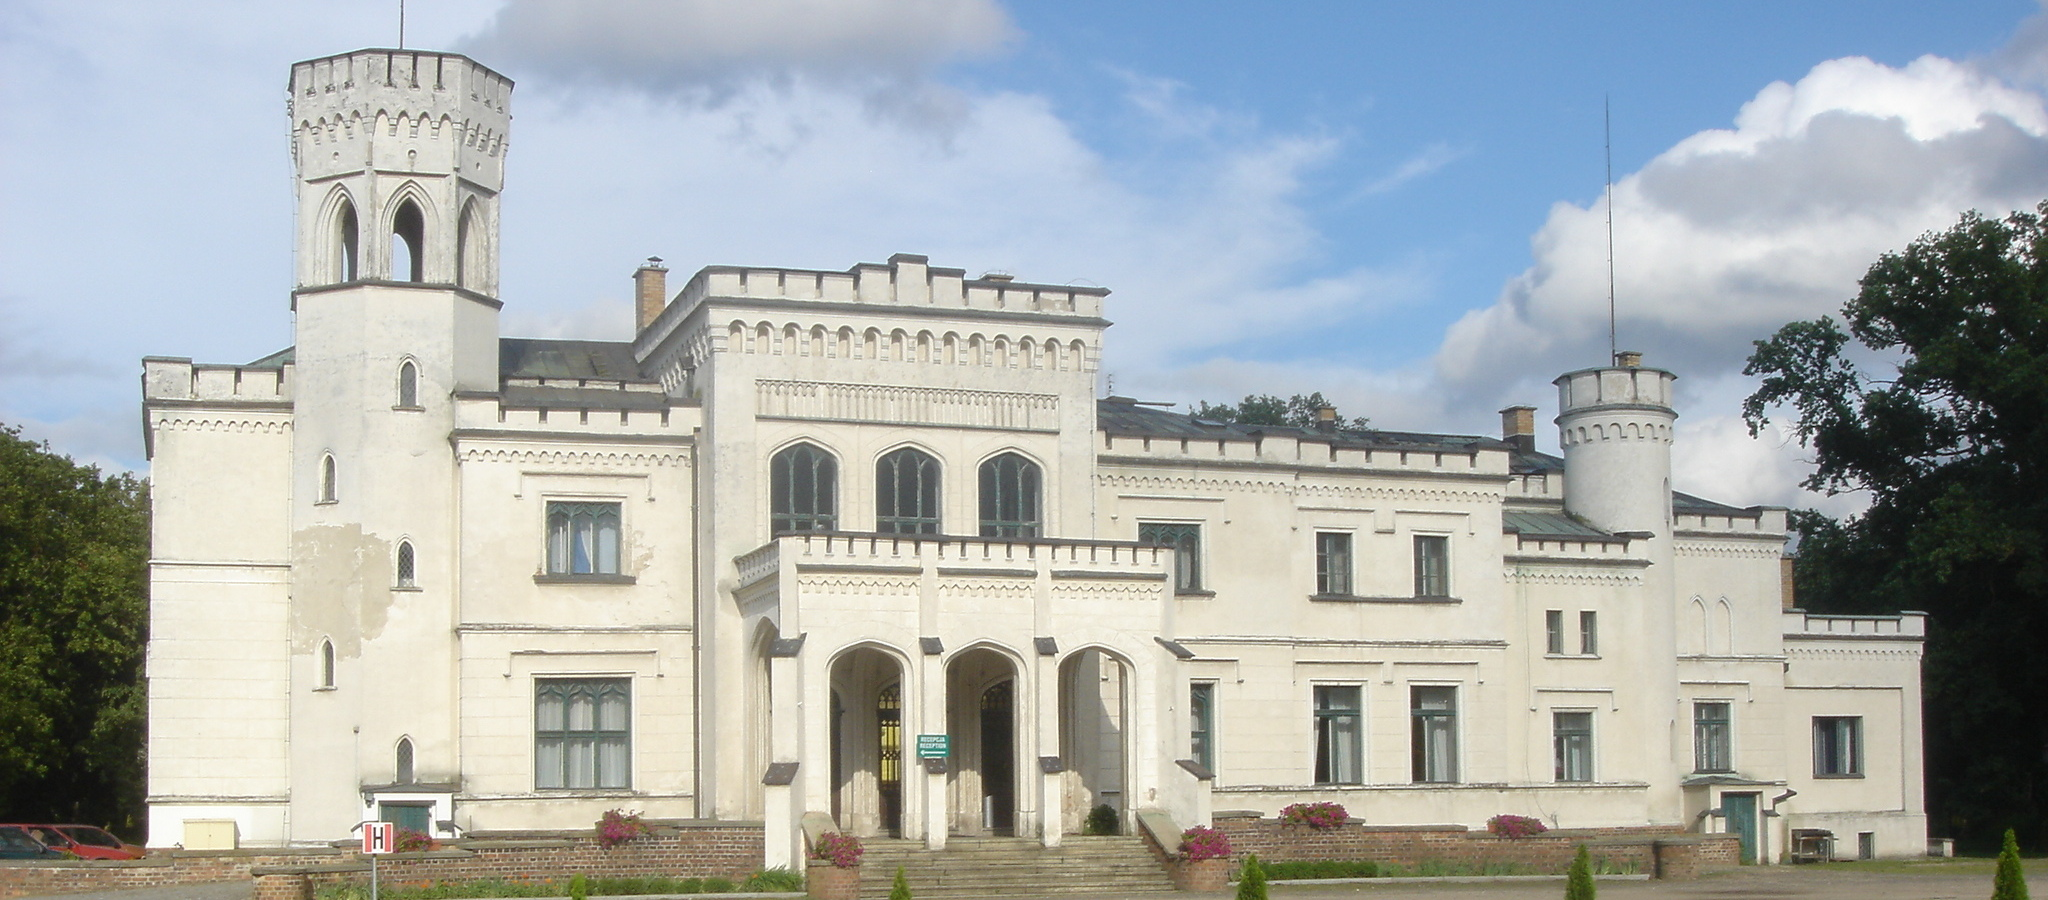
\includegraphics[width=.7\linewidth]{figs/bedlewo-c}

  \medskip
\end{center}

\begin{minipage}[t]{.473\linewidth}
  \nfont%
  Since 1994, the RAMiCS conference series has been the main venue for
  research on relation algebras, Kleene algebras and similar algebraic
  formalisms, and their applications as conceptual and methodological
  tools in computer science and beyond.

  \medskip

  Theoretical aspects include semigroups, residuated lattices,
  semirings, Kleene algebras, relation algebras, quantales and other
  algebras; their connections with program logics and other logics;
  their use in the theories of automata, concurrency, formal
  languages, games, networks and programming languages; the
  development of algebraic, algorithmic, category-theoretic,
  coalgebraic and proof-theoretic methods for these theories; their
  formalisation with theorem provers.

  \medskip

  Applications include tools and techniques for program correctness,
  specification and verification; quantitative and qualitative models
  and semantics of computing systems and processes; algorithm design,
  automated reasoning, network protocol analysis, social choice,
  optimisation and control.

  \bigskip

  {\Large \bf Call for Papers}

  \smallskip

  We invite original submissions in the general field of algebraic
  structures relevant to computer science and on applications of such
  algebras.  Submissions must be unpublished, not under review for
  publication elsewhere and provide sufficient information to judge
  their merits.
\end{minipage}
\hfill
\begin{minipage}[t]{.43\linewidth}
  \nfont%
  The proceedings of RAMiCS 2026 will be published in an LNCS volume
  by Springer.  As for earlier RAMiCS conferences, we intend to
  publish a journal special issue with revised and extended versions
  of a selection of the best papers.

  % \hfill {\Large \bf Invited Speakers}

  % \medskip

  % \begin{minipage}{.2\linewidth}
  %   \includegraphics[width=\linewidth, trim=0 30 0 0, clip]{kowalski2}
  % \end{minipage}
  % \hfill
  % \begin{minipage}{.75\linewidth}
  %   \textbf{Tomasz Kowalski}

  %   Jagiellonian University in Kraków

  %   Poland
  % \end{minipage}

  % \medskip

  % % \begin{minipage}{1.0\linewidth}
  % %   \flushleft%
  % %   \textbf{Compositional synthesis of interconnected control systems}
  % % \end{minipage}
  
  % %\vspace{-2ex}
  % \begin{minipage}{.75\linewidth}
  %   \flushright%
  %   \textbf{Sarah Winter}

  %   IRIF, Université Paris Cité

  %   France
  % \end{minipage}
  % \hfill
  % \begin{minipage}{.2\linewidth}
  %   \includegraphics[width=\linewidth, trim=0 0 0 0, clip]{winter}
  % \end{minipage}

  % \medskip

  % % \begin{minipage}{1.0\linewidth}
  % %   \flushright%
  % %   \textbf{Underwater robotics: past, present, and future}
  % % \end{minipage}
  
  % %\vspace{-2ex}
  % \begin{minipage}{.2\linewidth}
  %   \includegraphics[width=\linewidth, trim=15pt 0 0 0, clip]{goncharov2}
  % \end{minipage}
  % \hfill
  % \begin{minipage}{.75\linewidth}
  %   \textbf{Sergey Goncharov}

  %   % Friedrich-Alexander
  %   University of Erlangen \& Nürnberg

  %   Germany
  % \end{minipage}

  % \medskip
  
  % \begin{minipage}{1.0\linewidth}
  %   \flushleft%
  %   \textbf{Swarms of mobile robots, towards safety with versatility}
  % \end{minipage}

  \vspace*{2ex}
  
  \hfill {\Large \bf Organization}

  \smallskip

  \hfill \textbf{Uli Fahrenberg}, Paris-Saclay

  \hfill University, France

  \hfill \textbf{Wesley Fussner}, Czech Academy of

  \hfill Sciences, Prague, Czechia

  \hfill \textbf{Luigi Santocanale}, Aix-Marseille

  \hfill University, France

  \bigskip

  \hfill {\Large \bf Program Committee}

  \medskip

Henning Basold,
Manuel Bodirsky,
Andrew Craig,
Roland Glück,
Damas Gruska,
Walter Guttman,
Robin Hirsch,
Peter Höfner,
Marcel Jackson,
Ali Jaoua,
Peter Jipsen,
Tobias Kappé,
Bartek Klin,
Tomasz Kowalski,
Stepan Kuznetsov,
Sławek Lasota,
Ioana Leustean,
Roger Maddux,
Nelma Moreira,
Eugenia Ternovska,
Sara Ugolini,
Michael Winter,
Krzysztof Ziemiański,
Jas Šemrl
  
  \bigskip
  
  \hfill
  {\Large \bf Important Dates}

  \smallskip

  \hfill Abstract Submission: \textbf{1 November 2025}
  
  \hfill Paper Submission: \textbf{6 November 2025}
  
  % Author Notification: 20 January 2026

  %Final Version: 1 June 2024

  \vspace{8ex}

  \hspace*{-15ex} {\fontsize{30}{40}\selectfont https://ramics-conf.github.io/2026/}

  \vspace*{-2ex}

\end{minipage}

\end{document}
